\section{Multi-head Latent Attention (MLA)}
\label{sec:mla}

FlashAttention解决了训练时注意力矩阵的IO瓶颈,但推理时还存在另一个内存挑战:\textbf{KV Cache}。自回归生成需要缓存所有历史token的Key和Value向量,随着上下文长度增加,这部分内存占用可能超过模型参数本身。

Multi-head Latent Attention(MLA)是DeepSeek-V2~\citep{deepseek2024v2}针对这一问题提出的解决方案。其核心洞察是:虽然每个注意力头需要独立的K和V,但它们可能存在\textbf{低秩结构}——即可以从一个共享的低维"潜在向量"中恢复。这种压缩不同于GQA/MQA的强制共享,而是让网络学习最优的压缩方式。

\subsection{背景与目标}

\subsubsection{KV Cache的挑战}

如第~\ref{sec:transformer_math}节所述,自回归生成时需要缓存历史的K和V:
\begin{equation}
    \text{KV Cache Size} = 2 \times B \times S \times L \times n_h \times d_h \times \text{bytes}
\end{equation}

对于大模型(如$n_h = 128$,$d_h = 128$),KV Cache成为长上下文推理的主要内存瓶颈。

\subsubsection{现有方案的局限}

\begin{table}[htbp]
\centering
\caption{KV Cache优化方案对比}
\label{tab:kv_cache_methods}
\begin{tabular}{lccc}
\toprule
Method & KV Cache Size & Performance & 原理 \\
\midrule
MHA & $2 n_h d_h$ & 最优 & 每头独立KV \\
GQA & $2 \frac{n_h}{g} d_h$ & 轻微下降 & $g$个Q头共享KV \\
MQA & $2 d_h$ & 明显下降 & 所有头共享KV \\
\textbf{MLA} & $d_c + d_h^R$ & \textbf{接近MHA} & 低秩压缩 \\
\bottomrule
\end{tabular}
\end{table}

GQA/MQA通过共享KV头来减少缓存,但这种强制共享往往损害模型性能。MLA的核心洞察是:\textbf{KV可以从一个低维潜在向量中恢复},而不必显式共享。

\subsection{MLA核心原理}

\subsubsection{低秩压缩思想}

MLA的核心思想是将高维的Key和Value压缩到一个共享的低维潜在向量(latent vector),推理时从该向量恢复K和V。

\begin{figure}[htbp]
\centering
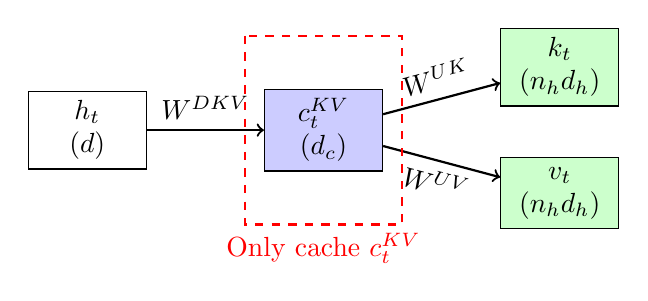
\begin{tikzpicture}[
    box/.style={rectangle, draw, minimum width=1.5cm, minimum height=0.8cm, align=center},
    arrow/.style={->, thick}
]
    % Input
    \node[box] (h) at (0,0) {$\bm{h}_t$\\$(d)$};

    % Compression
    \node[box, fill=blue!20] (c) at (3,0) {$\bm{c}_t^{KV}$\\$(d_c)$};

    % Decompression
    \node[box, fill=green!20] (k) at (6,0.8) {$\bm{k}_t$\\$(n_h d_h)$};
    \node[box, fill=green!20] (v) at (6,-0.8) {$\bm{v}_t$\\$(n_h d_h)$};

    % Arrows
    \draw[arrow] (h) -- node[above] {$W^{DKV}$} (c);
    \draw[arrow] (c) -- node[above, sloped] {$W^{UK}$} (k);
    \draw[arrow] (c) -- node[below, sloped] {$W^{UV}$} (v);

    % Cache indicator
    \draw[dashed, red, thick] (2,1.2) rectangle (4,-1.2);
    \node[red] at (3,-1.5) {Only cache $\bm{c}_t^{KV}$};
\end{tikzpicture}
\caption{MLA的KV压缩与恢复。只需缓存低维的$\bm{c}_t^{KV}$,K和V在计算时动态恢复。}
\label{fig:mla_compression}
\end{figure}

\subsection{数学公式}

\subsubsection{KV的低秩压缩}

对于输入 $\bm{h}_t \in \R^d$,首先压缩到潜在向量:
\begin{equation}
    \bm{c}_t^{KV} = W^{DKV} \bm{h}_t
    \label{eq:mla_compress}
\end{equation}
其中 $W^{DKV} \in \R^{d_c \times d}$ 是下投影矩阵,$d_c \ll n_h d_h$ 是压缩维度。

从潜在向量恢复K和V:
\begin{align}
    \bm{k}_t^C &= W^{UK} \bm{c}_t^{KV} \label{eq:mla_k} \\
    \bm{v}_t^C &= W^{UV} \bm{c}_t^{KV} \label{eq:mla_v}
\end{align}
其中 $W^{UK}, W^{UV} \in \R^{n_h d_h \times d_c}$ 是上投影矩阵。

\subsubsection{Query的低秩压缩}

类似地,Query也可以进行低秩压缩(主要用于减少训练时的激活内存):
\begin{align}
    \bm{c}_t^Q &= W^{DQ} \bm{h}_t \\
    \bm{q}_t^C &= W^{UQ} \bm{c}_t^Q
\end{align}
其中 $W^{DQ} \in \R^{d_c' \times d}$,$W^{UQ} \in \R^{n_h d_h \times d_c'}$。

\subsubsection{Decoupled RoPE}

RoPE需要在每个位置应用旋转,但如果直接对压缩后的$\bm{c}_t^{KV}$应用RoPE,会破坏后续的权重吸收优化。MLA采用\textbf{解耦RoPE}(Decoupled RoPE)策略:

\begin{enumerate}
    \item 将每个注意力头分为两部分:
    \begin{itemize}
        \item \textbf{内容部分}($d_h^C$维):从压缩向量恢复,\textbf{不}应用RoPE
        \item \textbf{位置部分}($d_h^R$维):额外投影,应用RoPE
    \end{itemize}

    \item 最终的Q和K为两部分的拼接:
    \begin{align}
        \bm{q}_t &= [\bm{q}_t^C; \text{RoPE}(\bm{q}_t^R, t)] \\
        \bm{k}_t &= [\bm{k}_t^C; \text{RoPE}(\bm{k}_t^R, t)]
    \end{align}
\end{enumerate}

其中位置部分的计算为:
\begin{align}
    \bm{q}_t^R &= W^{QR} \bm{c}_t^Q \\
    \bm{k}_t^R &= W^{KR} \bm{h}_t
\end{align}

\begin{remark}[为什么需要Decoupled RoPE]
RoPE是位置相关的:$\text{RoPE}(\bm{x}, t)$ 依赖于位置 $t$。如果对$\bm{c}_t^{KV}$应用RoPE再恢复K,则:
\[
    \bm{k}_t = W^{UK} \cdot \text{RoPE}(\bm{c}_t^{KV}, t)
\]
此时$W^{UK}$无法被吸收到$W^Q$中(因为RoPE在中间)。Decoupled策略将RoPE隔离到单独的维度,保留了权重吸收的可能性。
\end{remark}

\subsubsection{权重吸收}

MLA的一个关键优化是\textbf{权重吸收}(Weight Absorption)。由于压缩和恢复之间没有非线性激活,矩阵可以合并:

\paragraph{Query-Key吸收}
注意力分数的计算:
\begin{align}
    \bm{q}_t^{C\top} \bm{k}_s^C &= (\bm{c}_t^Q)^\top (W^{UQ})^\top W^{UK} \bm{c}_s^{KV} \\
    &= (\bm{c}_t^Q)^\top \underbrace{W^{QK}}_{\text{absorbed}} \bm{c}_s^{KV}
\end{align}
其中 $W^{QK} = (W^{UQ})^\top W^{UK} \in \R^{d_c' \times d_c}$。

\paragraph{Output-Value吸收}
输出投影的计算:
\begin{align}
    W^O \bm{v}_t^C &= W^O W^{UV} \bm{c}_t^{KV} \\
    &= \underbrace{W^{OV}}_{\text{absorbed}} \bm{c}_t^{KV}
\end{align}
其中 $W^{OV} = W^O W^{UV} \in \R^{d \times d_c}$。

\paragraph{推理流程}
权重吸收后,推理时:
\begin{enumerate}
    \item 缓存 $\bm{c}_t^{KV}$ 和 $\bm{k}_t^R$(位置部分)
    \item 用 $W^{QK}$ 直接计算内容部分的注意力分数
    \item 用吸收后的 $W^{OV}$ 计算输出
\end{enumerate}

\subsection{KV Cache分析}

\begin{table}[htbp]
\centering
\caption{MLA的KV Cache对比(per token per layer)}
\label{tab:mla_cache}
\begin{tabular}{lcc}
\toprule
Method & Cache Elements & DeepSeek-V2 (具体值) \\
\midrule
MHA & $2 n_h d_h$ & $2 \times 128 \times 128 = 32768$ \\
GQA (8组) & $2 \times 8 \times d_h$ & $2 \times 8 \times 128 = 2048$ \\
\textbf{MLA} & $d_c + d_h^R$ & $512 + 64 = 576$ \\
\bottomrule
\end{tabular}
\end{table}

DeepSeek-V2的配置:$d_c = 512$,$d_h^R = 64$,压缩比达到 $\frac{32768}{576} \approx \mathbf{56.9\times}$。

\subsection{PyTorch实现}

以下是MLA的简化PyTorch实现:

\begin{lstlisting}[language=Python, caption={MLA核心实现}]
import torch
import torch.nn as nn
import torch.nn.functional as F

class MultiHeadLatentAttention(nn.Module):
    def __init__(
        self,
        d_model: int,      # 模型维度
        n_heads: int,      # 注意力头数
        d_c: int,          # KV压缩维度
        d_c_q: int,        # Q压缩维度
        d_head_r: int,     # RoPE维度/头
    ):
        super().__init__()
        self.n_heads = n_heads
        self.d_head = d_model // n_heads
        self.d_c = d_c
        self.d_head_r = d_head_r

        # KV compression
        self.W_dkv = nn.Linear(d_model, d_c, bias=False)
        self.W_uk = nn.Linear(d_c, d_model, bias=False)
        self.W_uv = nn.Linear(d_c, d_model, bias=False)

        # Q compression
        self.W_dq = nn.Linear(d_model, d_c_q, bias=False)
        self.W_uq = nn.Linear(d_c_q, d_model, bias=False)

        # Decoupled RoPE projections
        self.W_qr = nn.Linear(d_c_q, n_heads * d_head_r, bias=False)
        self.W_kr = nn.Linear(d_model, n_heads * d_head_r, bias=False)

        # Output projection
        self.W_o = nn.Linear(d_model, d_model, bias=False)

    def forward(self, x, rope_fn, kv_cache=None):
        B, T, D = x.shape

        # KV compression: only c_kv needs caching
        c_kv = self.W_dkv(x)  # (B, T, d_c)

        # Decoupled RoPE keys
        k_r = self.W_kr(x)    # (B, T, n_heads * d_head_r)
        k_r = rope_fn(k_r)    # Apply RoPE

        # Handle KV cache
        if kv_cache is not None:
            c_kv_cached, k_r_cached = kv_cache
            c_kv = torch.cat([c_kv_cached, c_kv], dim=1)
            k_r = torch.cat([k_r_cached, k_r], dim=1)
        new_cache = (c_kv, k_r)

        # Q compression
        c_q = self.W_dq(x)    # (B, T, d_c_q)
        q_c = self.W_uq(c_q)  # (B, T, D) - content part
        q_r = self.W_qr(c_q)  # (B, T, n_heads * d_head_r) - RoPE part
        q_r = rope_fn(q_r)

        # Reconstruct K, V from compressed cache
        k_c = self.W_uk(c_kv)  # (B, S, D) - content part
        v = self.W_uv(c_kv)    # (B, S, D)

        # Reshape for multi-head attention
        q_c = q_c.view(B, T, self.n_heads, self.d_head)
        k_c = k_c.view(B, -1, self.n_heads, self.d_head)
        v = v.view(B, -1, self.n_heads, self.d_head)
        q_r = q_r.view(B, T, self.n_heads, self.d_head_r)
        k_r = k_r.view(B, -1, self.n_heads, self.d_head_r)

        # Concatenate content and RoPE parts
        q = torch.cat([q_c, q_r], dim=-1)  # (B, T, H, d_head + d_head_r)
        k = torch.cat([k_c, k_r], dim=-1)  # (B, S, H, d_head + d_head_r)

        # Scaled dot-product attention
        q, k, v = q.transpose(1,2), k.transpose(1,2), v.transpose(1,2)
        scale = (self.d_head + self.d_head_r) ** -0.5
        attn = F.softmax(q @ k.transpose(-2,-1) * scale, dim=-1)
        out = attn @ v  # (B, H, T, d_head)

        # Output projection
        out = out.transpose(1,2).reshape(B, T, D)
        out = self.W_o(out)

        return out, new_cache
\end{lstlisting}

\begin{remark}[实现优化]
上述代码为教学版本。实际部署时:
\begin{itemize}
    \item 权重吸收:预计算 $W^{QK} = (W^{UQ})^\top W^{UK}$ 和 $W^{OV} = W^O W^{UV}$
    \item Flash Attention:使用FlashAttention加速注意力计算
    \item 融合算子:将多个小矩阵乘法融合
\end{itemize}
\end{remark}

\subsection{MLA vs 其他方法}

\begin{table}[htbp]
\centering
\caption{注意力机制全面对比}
\label{tab:attention_comparison}
\begin{tabular}{lcccc}
\toprule
Feature & MHA & GQA & MQA & MLA \\
\midrule
KV Cache & $2n_h d_h$ & $2\frac{n_h}{g} d_h$ & $2 d_h$ & $d_c + d_h^R$ \\
参数量 & 基准 & 减少 & 最少 & 略增 \\
表达能力 & 最强 & 较强 & 较弱 & 接近MHA \\
推理延迟 & 高 & 中 & 低 & 中 \\
长上下文 & 受限 & 较好 & 好 & \textbf{最好} \\
\bottomrule
\end{tabular}
\end{table}

\paragraph{MLA的优势}
\begin{itemize}
    \item \textbf{极致压缩}:KV Cache减少93\%以上
    \item \textbf{性能保持}:不像GQA/MQA强制共享,而是学习最优压缩
    \item \textbf{长上下文友好}:128K上下文成为可能
\end{itemize}

\paragraph{MLA的代价}
\begin{itemize}
    \item \textbf{计算开销}:需要额外的压缩/恢复计算
    \item \textbf{实现复杂度}:Decoupled RoPE和权重吸收增加实现难度
    \item \textbf{训练成本}:低秩约束可能需要更多训练
\end{itemize}

\subsection{质量-效率权衡:何时使用MLA?}

MLA并非银弹。其56.9倍的压缩比来自于一个强假设:\textbf{K和V可以从512维潜在空间无损恢复}。这个假设在什么条件下成立?

\subsubsection{低秩假设的有效性}

考虑注意力模式的多样性需求。设任务需要 $r$ 种本质不同的注意力模式(如:局部依赖、长程依赖、语法结构、语义关联等),则KV表示至少需要 $r$ 个自由度。

\paragraph{压缩维度的下界}
若 $d_c < r$,则压缩会造成信息丢失。DeepSeek选择 $d_c = 512$,隐含假设是:常见NLP任务的注意力模式可以用不超过512维的空间表达。

\paragraph{任务依赖性}
不同任务对注意力多样性的需求不同:
\begin{itemize}
    \item \textbf{文本生成}:模式相对固定,低秩假设成立,MLA表现良好
    \item \textbf{代码理解}:需要追踪复杂的变量依赖和作用域,可能需要更高秩的表示
    \item \textbf{数学推理}:多步推理需要维持多条推理链,对注意力多样性要求高
\end{itemize}

\subsubsection{选择指南}

\begin{table}[htbp]
\centering
\caption{注意力机制选择指南}
\label{tab:attention_selection}
\begin{tabular}{lcc}
\toprule
场景 & 推荐方法 & 理由 \\
\midrule
长上下文推理 (>32K) & MLA & KV Cache是主要瓶颈 \\
短上下文、高吞吐 & GQA & 实现简单,开销低 \\
质量优先(小batch) & MHA & 无压缩损失 \\
代码/数学任务 & GQA或MHA & 注意力多样性需求高 \\
边缘设备部署 & MLA & 极致内存压缩 \\
\bottomrule
\end{tabular}
\end{table}

\paragraph{经验法则}
当 $\text{上下文长度} \times \text{batch size} > 10^6$ 时,KV Cache成为主要瓶颈,MLA的收益开始显现。对于短上下文或小batch推理,GQA的简单性可能更具优势。

\subsubsection{压缩比与质量的帕累托边界}

DeepSeek的消融实验表明,$d_c$ 的选择存在"甜点区":
\begin{itemize}
    \item $d_c < 256$:质量显著下降,压缩过度
    \item $d_c \in [256, 768]$:质量接近MHA,压缩有效
    \item $d_c > 768$:质量无进一步提升,压缩收益递减
\end{itemize}

$d_c = 512$ 处于帕累托最优附近——进一步压缩会损害质量,进一步扩大则浪费缓存空间。

\subsection{应用与扩展}

MLA已在以下模型中应用:
\begin{itemize}
    \item \textbf{DeepSeek-V2}:首次提出,236B参数MoE模型
    \item \textbf{DeepSeek-V3}:进一步优化,671B参数
    \item \textbf{DeepSeek-R1}:推理模型,继承MLA架构
\end{itemize}

\begin{remark}[MLA与MoE的协同]
MLA特别适合MoE架构:MoE的稀疏激活已经减少了计算量,而MLA进一步解决了内存瓶颈。两者结合使得DeepSeek-V2在保持高性能的同时,训练成本降低42.5\%。
\end{remark}
